\documentclass[tikz,border=10pt]{standalone}
% Shared look for every TikZ diagram. Load with \input{../../tools/tikz-style.tex}
\usepackage[T1]{fontenc}
\usepackage{lmodern}
\renewcommand{\sfdefault}{lmr}  % diagrams use the same serif as the text
\usetikzlibrary{arrows.meta, positioning, shapes.geometric, calc, fit, backgrounds}
\definecolor{cblue}{HTML}{4C78A8}
\definecolor{corange}{HTML}{F58518}
\definecolor{cgreen}{HTML}{54A24B}
\definecolor{cred}{HTML}{E45756}
\definecolor{cpurple}{HTML}{B279A2}
\definecolor{cgrey}{HTML}{6B6B6B}
\tikzset{
  every picture/.style={font=\sffamily, line width=1.2pt},
  box/.style={draw=#1, fill=#1!12, rounded corners=4pt, align=center, inner sep=7pt, minimum height=1.1cm},
  box/.default=cgrey,
  arrow/.style={-{Stealth[length=3mm]}, draw=cgrey, line width=1.4pt},
  title/.style={font=\sffamily\bfseries\Large},
  note/.style={font=\sffamily\small, text=cgrey, align=center},
}
\AtBeginDocument{\hyphenpenalty=10000 \exhyphenpenalty=10000}

\begin{document}
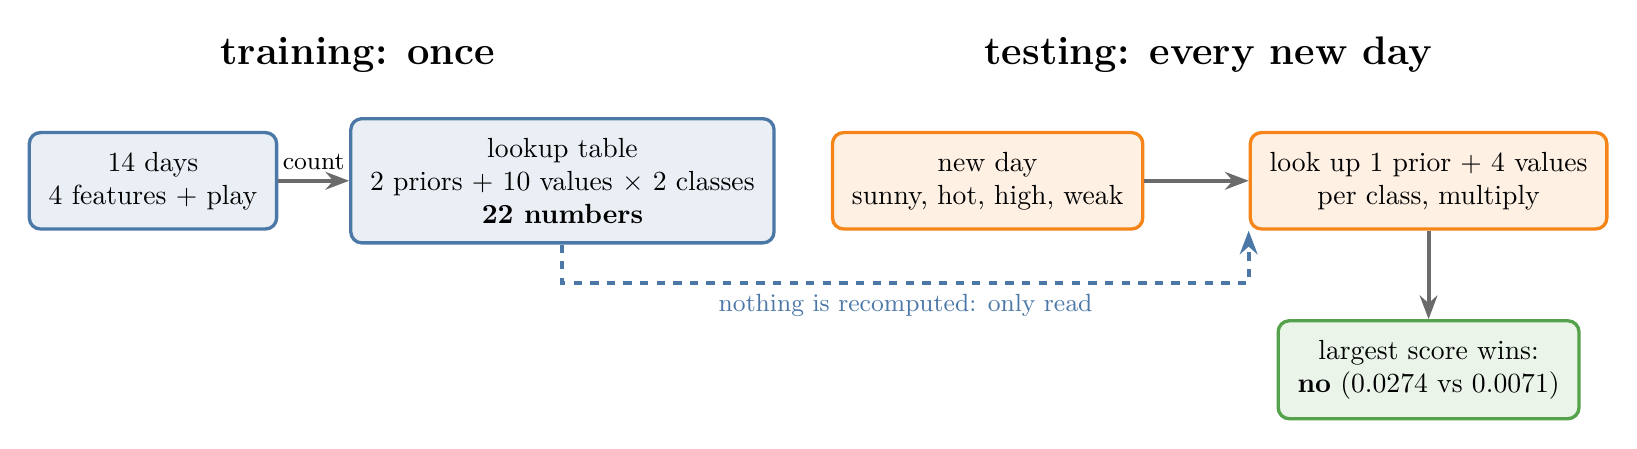
\begin{tikzpicture}[node distance=1.2cm and 1.3cm]
  \node[title] at (2.6,1.6) {training: once};
  \node[title] at (13.4,1.6) {testing: every new day};
  \node[box=cblue] (data) at (0,0) {14 days\\ 4 features + play};
  \node[box=cblue] (table) at (5.2,0) {lookup table\\ 2 priors + 10 values $\times$ 2 classes\\ \textbf{22 numbers}};
  \node[box=corange] (day) at (10.6,0) {new day\\ sunny, hot, high, weak};
  \node[box=corange] (mult) at (16.2,0) {look up 1 prior + 4 values\\ per class, multiply};
  \node[box=cgreen] (pred) at (16.2,-2.4) {largest score wins:\\ \textbf{no} (0.0274 vs 0.0071)};
  \draw[arrow] (data) -- node[above, font=\small] {count} (table);
  \draw[arrow] (day) -- (mult);
  \draw[arrow] (mult) -- (pred);
  \draw[arrow, cblue, dashed] (table.south) |- node[below, pos=0.75, font=\small, text=cblue] {nothing is recomputed: only read} (mult.south west |- 0,-1.3) -- (mult.south west);
\end{tikzpicture}
\end{document}
